% ============================================================
% Project 3: Alamouti STBC 2×1 MISO - Presentation
% Sorbonne Université - MU5EEF08 Wireless Communications
% ============================================================
\documentclass[aspectratio=169]{beamer}

% Theme
\usetheme{Madrid}
\usecolortheme{default}
\setbeamertemplate{navigation symbols}{}
\setbeamertemplate{footline}[frame number]

% Packages
\usepackage[utf8]{inputenc}
\usepackage[T1]{fontenc}
\usepackage{amsmath,amssymb}
\usepackage{graphicx}
\usepackage{booktabs}
\usepackage{tikz}
\usetikzlibrary{shapes.geometric, arrows, positioning, fit, backgrounds, calc}

% Graphics path
\graphicspath{{image/README/}}

% Title information
\title[Alamouti STBC]{Project 3: Alamouti STBC\\2×1 MISO Wireless Communication System}
\author{LI Yanbo \and Yasten Belaid}
\institute[Sorbonne]{Sorbonne Université\\MU5EEF08 - Wireless Communications}
\date{January 2026}

% ============================================================
\begin{document}

% ------------------------------------------------------------
% Title Slide
% ------------------------------------------------------------
\begin{frame}
  \titlepage
\end{frame}

% ------------------------------------------------------------
% Outline
% ------------------------------------------------------------
\begin{frame}{Outline}
  \tableofcontents
\end{frame}

% ============================================================
\section{Introduction}
% ============================================================

\begin{frame}{Project Objective}
  \begin{columns}
    \column{0.5\textwidth}
    \textbf{Goal:} Implement and evaluate \textbf{Alamouti STBC} for 2×1 MISO system
    
    \vspace{1em}
    \textbf{Key Features:}
    \begin{itemize}
      \item 16-QAM modulation
      \item Pilot-based channel estimation (LS)
      \item BER comparison: SISO vs Alamouti
    \end{itemize}
    
    \vspace{1em}
    \textbf{Extensions:}
    \begin{itemize}
      \item Rice channel (K-factor)
      \item TX spatial correlation ($\rho$)
      \item Doppler time-varying fading
    \end{itemize}
    
    \column{0.5\textwidth}
    \begin{block}{Alamouti Diversity Gain}
      \begin{itemize}
        \item SISO: Diversity order = 1
        \item Alamouti 2×1: Diversity order = 2
        \item $\Rightarrow$ \textbf{3-4 dB} SNR gain at high SNR
      \end{itemize}
    \end{block}
    
    \vspace{1em}
    \begin{block}{Project Structure}
      \scriptsize
      \begin{enumerate}
        \item \texttt{Main\_Alamouti\_Full\_Project.m}\\(Base implementation)
        \item \texttt{Main\_Alamouti\_Extensions.m}\\(Advanced extensions)
      \end{enumerate}
    \end{block}
  \end{columns}
\end{frame}

% ============================================================
% ============================================================
% PART I: BASE PROJECT (Main_Alamouti_Full_Project.m)
% ============================================================
% ============================================================

\section{Base Project: System Model}

\begin{frame}{System Block Diagram}
  \begin{figure}
    \centering
    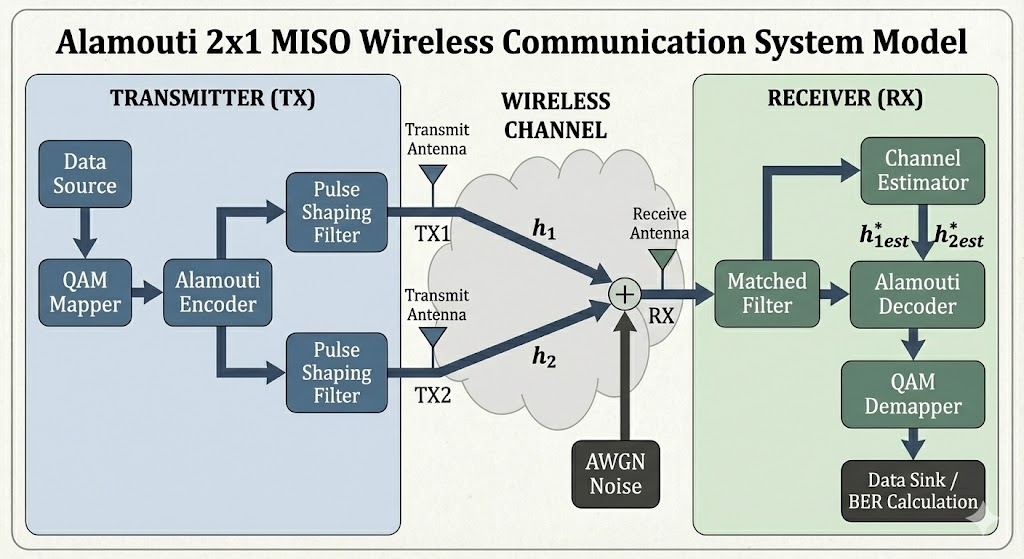
\includegraphics[width=0.68\textwidth]{System_Block_Diagram_Full.png}
    \caption{Alamouti 2×1 MISO Wireless Communication System}
  \end{figure}
\end{frame}

\begin{frame}{Alamouti Encoding (TX)}
  \begin{columns}
    \column{0.45\textwidth}
    \begin{figure}
      \centering
      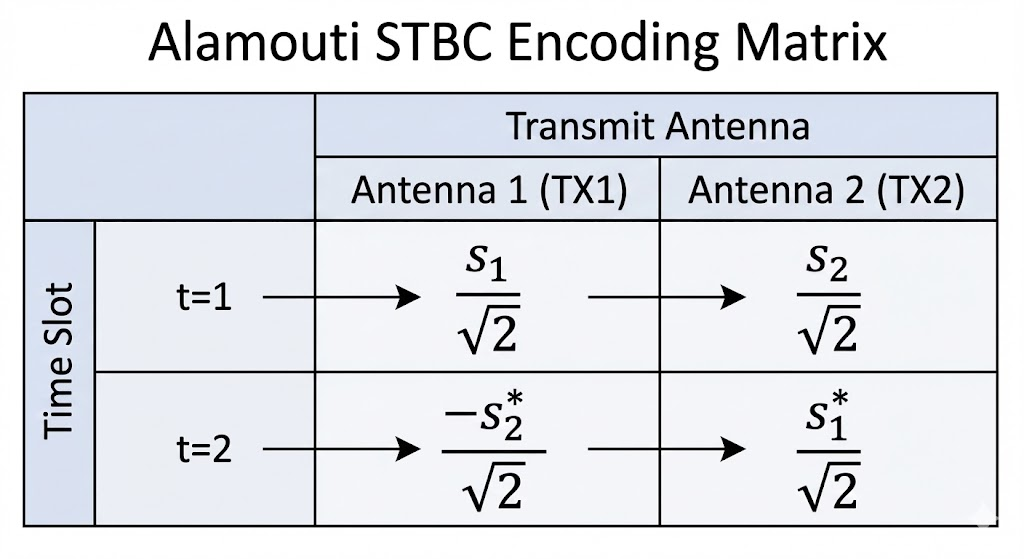
\includegraphics[width=\textwidth]{Alamouti_Encoding_Matrix.png}
    \end{figure}
    
    \column{0.55\textwidth}
    \textbf{Space-Time Block Code Matrix:}
    \[
    \mathbf{X} = \frac{1}{\sqrt{2}} \begin{bmatrix} s_1 & -s_2^* \\ s_2 & s_1^* \end{bmatrix}
    \]
    
    \vspace{0.5em}
    \begin{itemize}
      \item Row = Antenna (TX1, TX2)
      \item Column = Time slot ($t_1$, $t_2$)
      \item $\frac{1}{\sqrt{2}}$: Power normalization
    \end{itemize}
    
    \vspace{0.5em}
    \textbf{Received signals:}
    \begin{align*}
      y_1 &= \frac{1}{\sqrt{2}}(h_1 s_1 + h_2 s_2) + n_1 \\
      y_2 &= \frac{1}{\sqrt{2}}(-h_1 s_2^* + h_2 s_1^*) + n_2
    \end{align*}
  \end{columns}
\end{frame}

\begin{frame}{Alamouti Decoding (RX)}
  \begin{columns}
    \column{0.5\textwidth}
    \begin{figure}
      \centering
      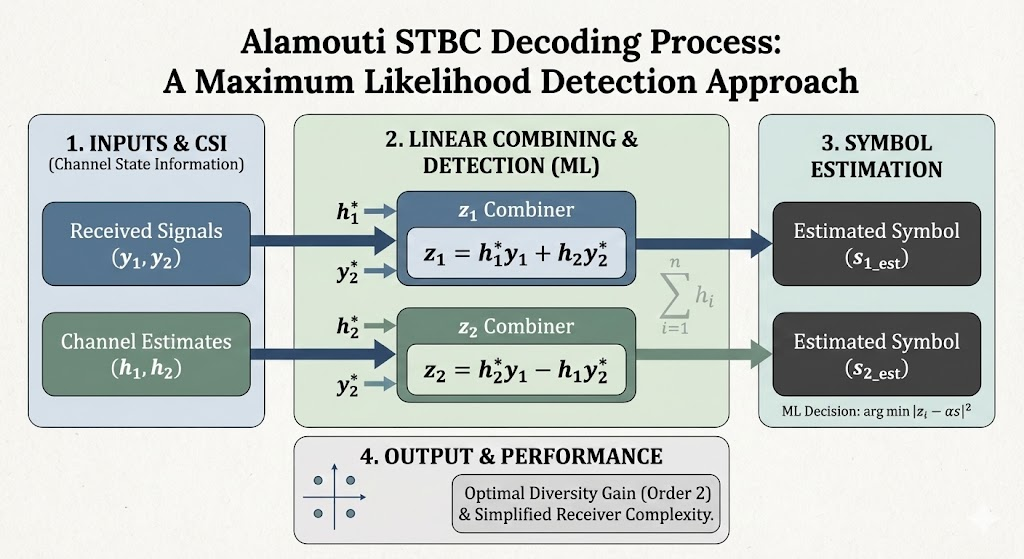
\includegraphics[width=\textwidth]{Alamouti_Decoding_Process.png}
    \end{figure}
    
    \column{0.5\textwidth}
    \textbf{Linear Combining:}
    \begin{align*}
      z_1 &= \frac{1}{\sqrt{2}}(h_1^* y_1 + h_2 y_2^*) \\
      z_2 &= \frac{1}{\sqrt{2}}(h_2^* y_1 - h_1 y_2^*)
    \end{align*}
    
    \vspace{0.5em}
    \textbf{After simplification:}
    \[
    z_i = \underbrace{\frac{|h_1|^2 + |h_2|^2}{2}}_{\alpha} \cdot s_i + \tilde{n}_i
    \]
    
    \vspace{0.5em}
    \textbf{Equalization:}
    \[
    \hat{s}_i = \frac{z_i}{\alpha}
    \]
  \end{columns}
\end{frame}

\begin{frame}{Orthogonal Pilot-Based Channel Estimation}
  \begin{figure}
    \centering
    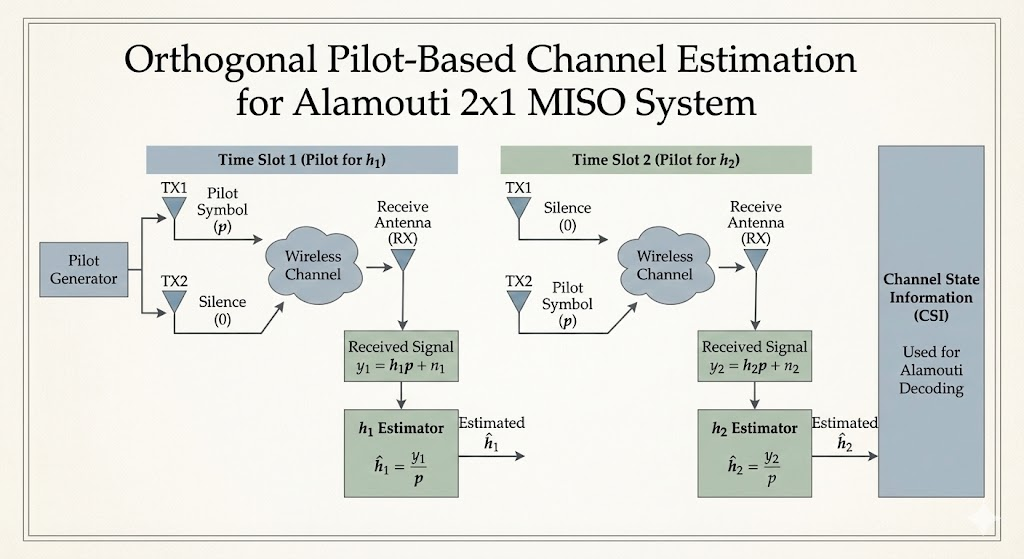
\includegraphics[width=0.75\textwidth]{Orthogonal_Pilot_Channel_Estimation.png}
  \end{figure}
  
  \vspace{-0.5em}
  \begin{columns}
    \column{0.5\textwidth}
    \centering
    \textbf{Time Slot 1-10:} TX1 sends pilot, TX2 silent\\
    $\hat{h}_1 = \frac{1}{N_p}\sum_{i=1}^{N_p} \frac{y_i}{p_i}$
    
    \column{0.5\textwidth}
    \centering
    \textbf{Time Slot 11-20:} TX1 silent, TX2 sends pilot\\
    $\hat{h}_2 = \frac{1}{N_p}\sum_{i=1}^{N_p} \frac{y_i}{p_i}$
  \end{columns}
\end{frame}

% ------------------------------------------------------------
\section{Base Project: Code Structure}
% ------------------------------------------------------------

\begin{frame}{Main\_Alamouti\_Full\_Project.m: Two-Part Structure}
  \centering
  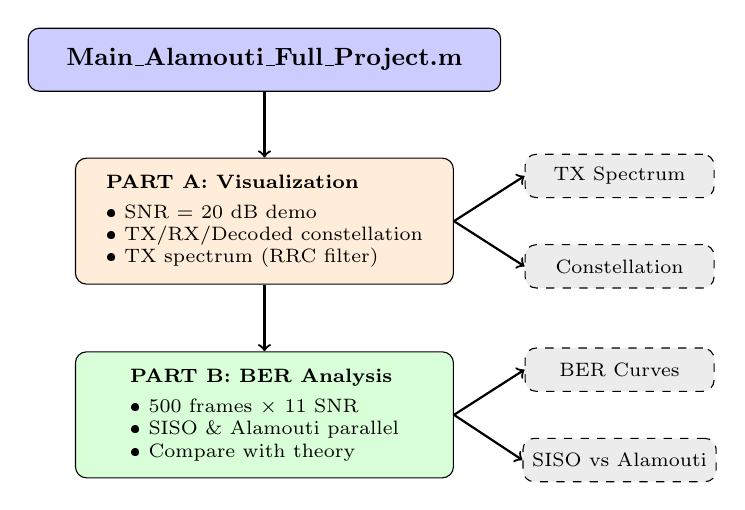
\begin{tikzpicture}[
    scale=0.82,
    mainbox/.style={rectangle, draw, rounded corners, fill=blue!20, minimum width=6cm, minimum height=0.8cm, font=\small\bfseries},
    partbox/.style={rectangle, draw, rounded corners, minimum width=4.8cm, minimum height=1.6cm, align=left, font=\scriptsize},
    outbox/.style={rectangle, draw, dashed, rounded corners, fill=gray!15, minimum width=2.4cm, minimum height=0.55cm, align=center, font=\scriptsize},
    arrow/.style={->, thick}
  ]
    % Title - aligned with Part A and Part B (x = -2)
    \node[mainbox] (title) at (-2,0) {Main\_Alamouti\_Full\_Project.m};
    
    % Part A
    \node[partbox, fill=orange!15] (partA) at (-2,-2.5) {
      \textbf{PART A: Visualization}\\[3pt]
      • SNR = 20 dB demo\\
      • TX/RX/Decoded constellation\\
      • TX spectrum (RRC filter)
    };
    
    % Part A outputs - further right
    \node[outbox] (outA1) at (3.5,-1.8) {TX Spectrum};
    \node[outbox] (outA2) at (3.5,-3.2) {Constellation};
    
    % Part B
    \node[partbox, fill=green!15] (partB) at (-2,-5.5) {
      \textbf{PART B: BER Analysis}\\[3pt]
      • 500 frames $\times$ 11 SNR\\
      • SISO \& Alamouti parallel\\
      • Compare with theory
    };
    
    % Part B outputs - further right
    \node[outbox] (outB1) at (3.5,-4.8) {BER Curves};
    \node[outbox] (outB2) at (3.5,-6.2) {SISO vs Alamouti};
    
    % Arrow from title to Part A
    \draw[arrow] (title.south) -- (partA.north);
    
    % Arrow from Part A to Part B
    \draw[arrow] (partA.south) -- (partB.north);
    
    % Arrows from Part A to outputs (horizontal)
    \draw[arrow] (partA.east) -- (outA1.west);
    \draw[arrow] (partA.east) -- (outA2.west);
    
    % Arrows from Part B to outputs (horizontal)
    \draw[arrow] (partB.east) -- (outB1.west);
    \draw[arrow] (partB.east) -- (outB2.west);
  \end{tikzpicture}
  
  \vspace{0.3em}
  \begin{block}{Key Design}
    \scriptsize
    Both SISO and Alamouti use \textbf{identical} parameters (16-QAM, pilots, SNR) for fair comparison.
  \end{block}
\end{frame}

\begin{frame}{Base Project: Complete TX-RX Processing Chain}
  \centering
  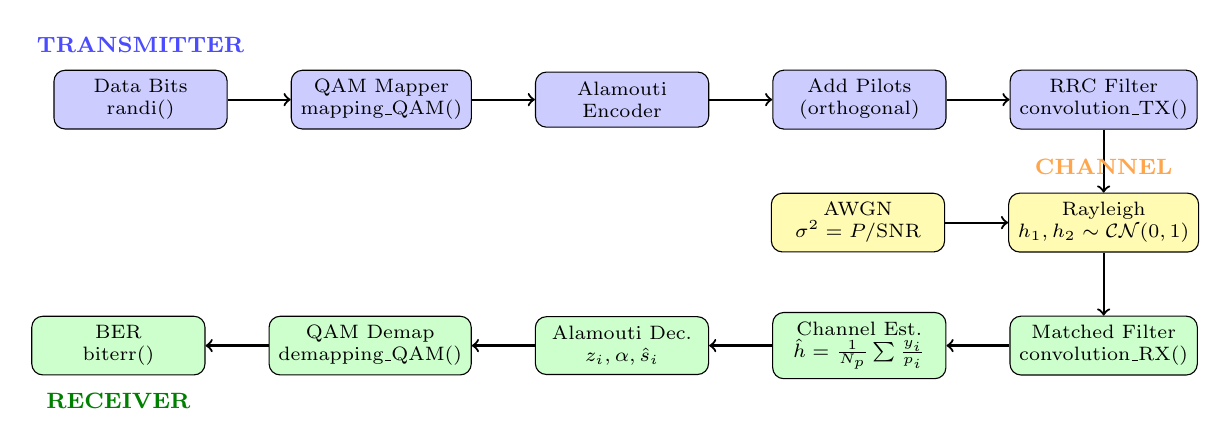
\begin{tikzpicture}[
    node distance=0.4cm and 0.8cm,
    box/.style={rectangle, draw, rounded corners, minimum width=2.2cm, minimum height=0.7cm, align=center, font=\scriptsize},
    txbox/.style={box, fill=blue!20},
    chbox/.style={box, fill=yellow!30},
    rxbox/.style={box, fill=green!20},
    arrow/.style={->, thick}
  ]
    % TX Chain
    \node[txbox] (bits) {Data Bits\\randi()};
    \node[txbox, right=of bits] (qam) {QAM Mapper\\mapping\_QAM()};
    \node[txbox, right=of qam] (ala_enc) {Alamouti\\Encoder};
    \node[txbox, right=of ala_enc] (pilot) {Add Pilots\\(orthogonal)};
    \node[txbox, right=of pilot] (rrc_tx) {RRC Filter\\convolution\_TX()};
    
    % Channel
    \node[chbox, below=0.8cm of rrc_tx] (channel) {Rayleigh\\$h_1, h_2 \sim \mathcal{CN}(0,1)$};
    \node[chbox, left=of channel] (noise) {AWGN\\$\sigma^2 = P/\text{SNR}$};
    
    % RX Chain
    \node[rxbox, below=0.8cm of channel] (rrc_rx) {Matched Filter\\convolution\_RX()};
    \node[rxbox, left=of rrc_rx] (ch_est) {Channel Est.\\$\hat{h}=\frac{1}{N_p}\sum\frac{y_i}{p_i}$};
    \node[rxbox, left=of ch_est] (ala_dec) {Alamouti Dec.\\$z_i, \alpha, \hat{s}_i$};
    \node[rxbox, left=of ala_dec] (deqam) {QAM Demap\\demapping\_QAM()};
    \node[rxbox, left=of deqam] (ber) {BER\\biterr()};
    
    % Arrows
    \draw[arrow] (bits) -- (qam);
    \draw[arrow] (qam) -- (ala_enc);
    \draw[arrow] (ala_enc) -- (pilot);
    \draw[arrow] (pilot) -- (rrc_tx);
    \draw[arrow] (rrc_tx) -- (channel);
    \draw[arrow] (noise) -- (channel);
    \draw[arrow] (channel) -- (rrc_rx);
    \draw[arrow] (rrc_rx) -- (ch_est);
    \draw[arrow] (ch_est) -- (ala_dec);
    \draw[arrow] (ala_dec) -- (deqam);
    \draw[arrow] (deqam) -- (ber);
    
    % Labels
    \node[above=0.1cm of bits, font=\footnotesize\bfseries, blue!70] {TRANSMITTER};
    \node[above=0.1cm of channel, font=\footnotesize\bfseries, orange!70] {CHANNEL};
    \node[below=0.1cm of ber, font=\footnotesize\bfseries, green!50!black] {RECEIVER};
  \end{tikzpicture}
  
  \vspace{0.3em}
  \small
  \begin{columns}
    \column{0.5\textwidth}
    \textbf{Parameters:}
    \begin{itemize}
      \scriptsize
      \item 16-QAM: 4 bits/symbol
      \item 1000 data symbols/frame
      \item 10 pilot symbols (orthogonal)
    \end{itemize}
    
    \column{0.5\textwidth}
    \textbf{Frame Structure:}
    \begin{itemize}
      \scriptsize
      \item TX1: $[P, 0, \text{data}]$
      \item TX2: $[0, P, \text{data}]$
      \item Total: 20 pilots + 1000 data
    \end{itemize}
  \end{columns}
\end{frame}

% ------------------------------------------------------------
\section{Base Project: Simulation Results}
% ------------------------------------------------------------

\begin{frame}{TX Spectrum}
  \begin{columns}
    \column{0.6\textwidth}
    \begin{figure}
      \centering
      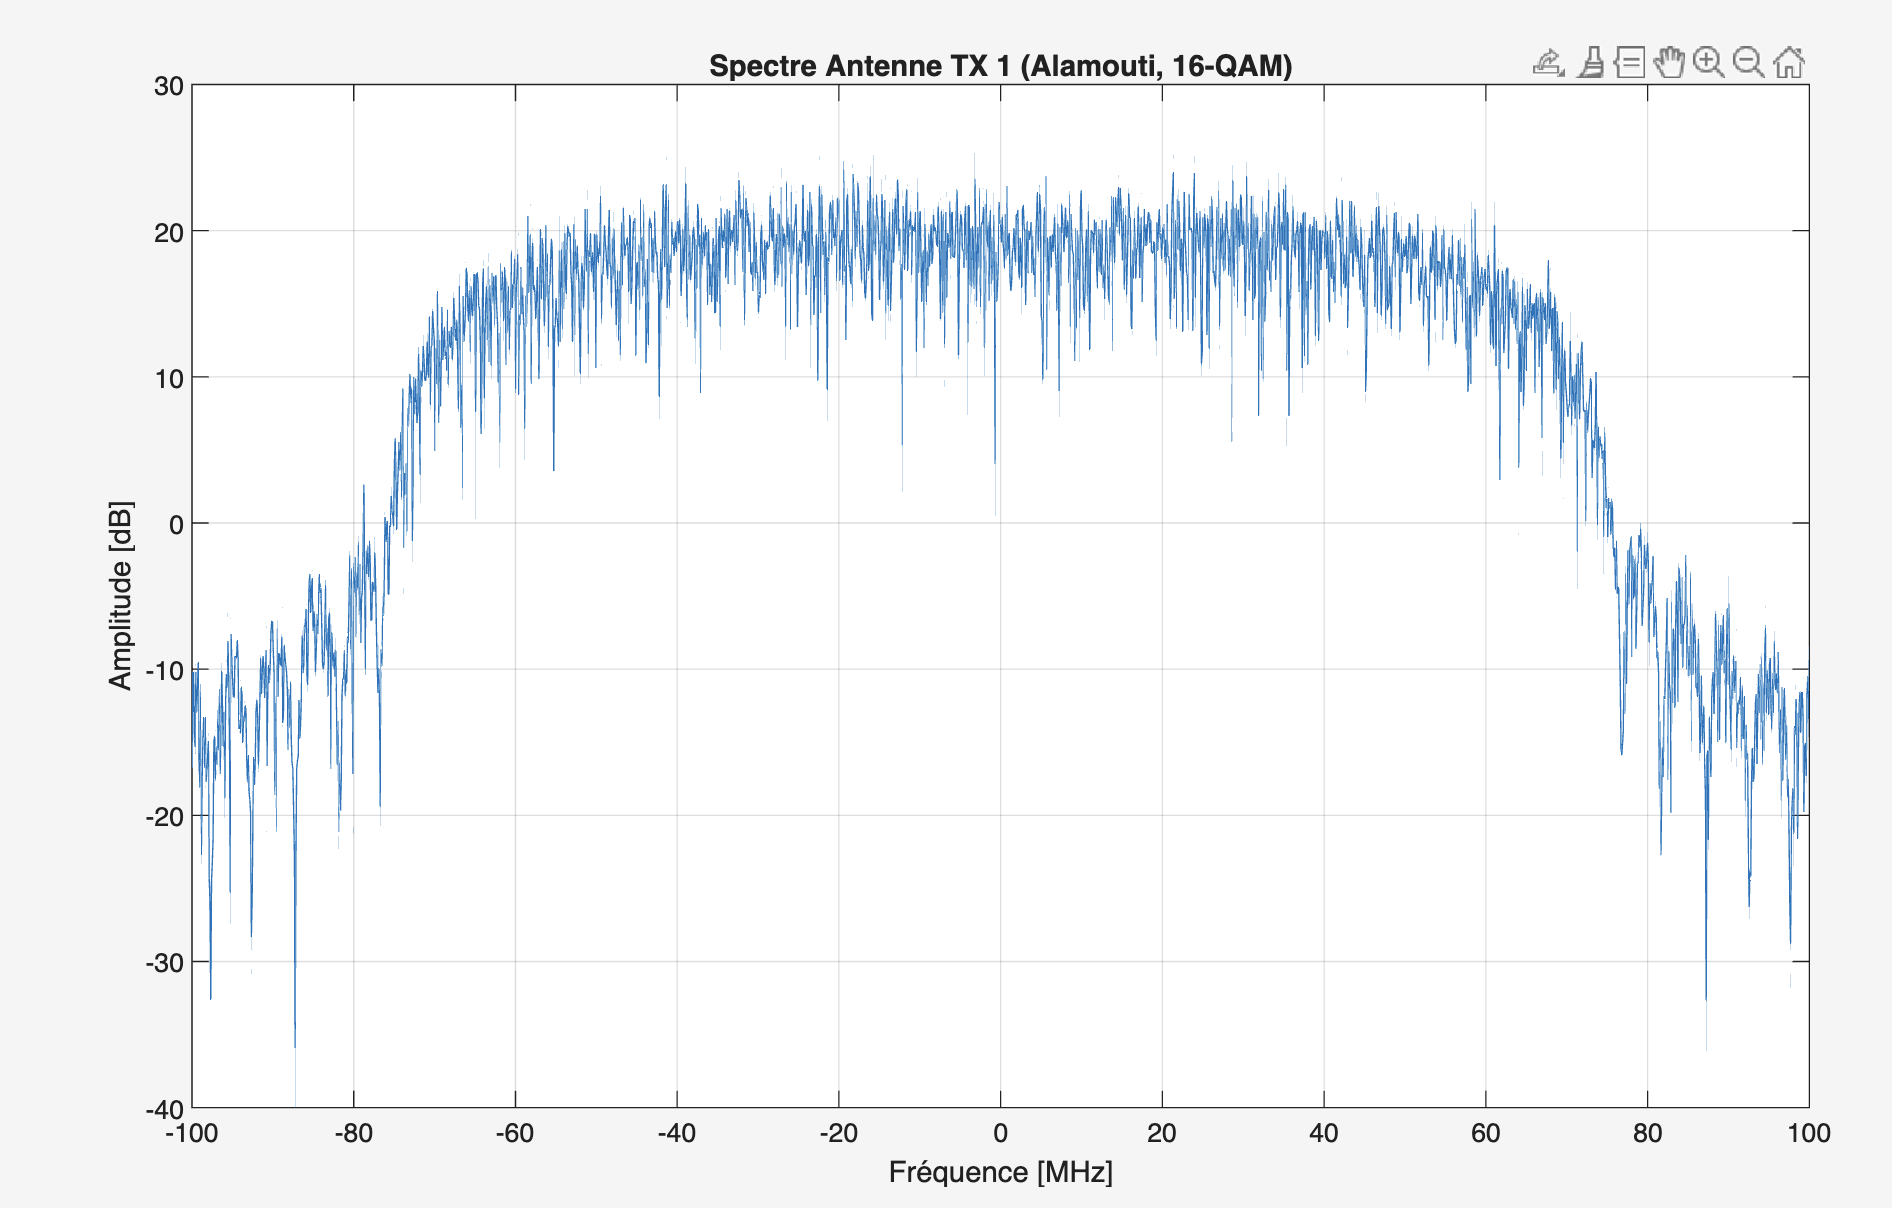
\includegraphics[width=\textwidth]{TX_Spectrum_Alamouti_16QAM.png}
    \end{figure}
    
    \column{0.4\textwidth}
    \textbf{Parameters:}
    \begin{itemize}
      \item Symbol rate: 100 Msym/s
      \item Roll-off: $\beta = 0.5$
      \item Bandwidth: $(1+\beta) R_s$\\= 150 MHz
    \end{itemize}
    
    \vspace{1em}
    \textbf{Filter:} Root Raised Cosine (RRC)
  \end{columns}
\end{frame}

\begin{frame}{Constellation Diagrams}
  \begin{figure}
    \centering
    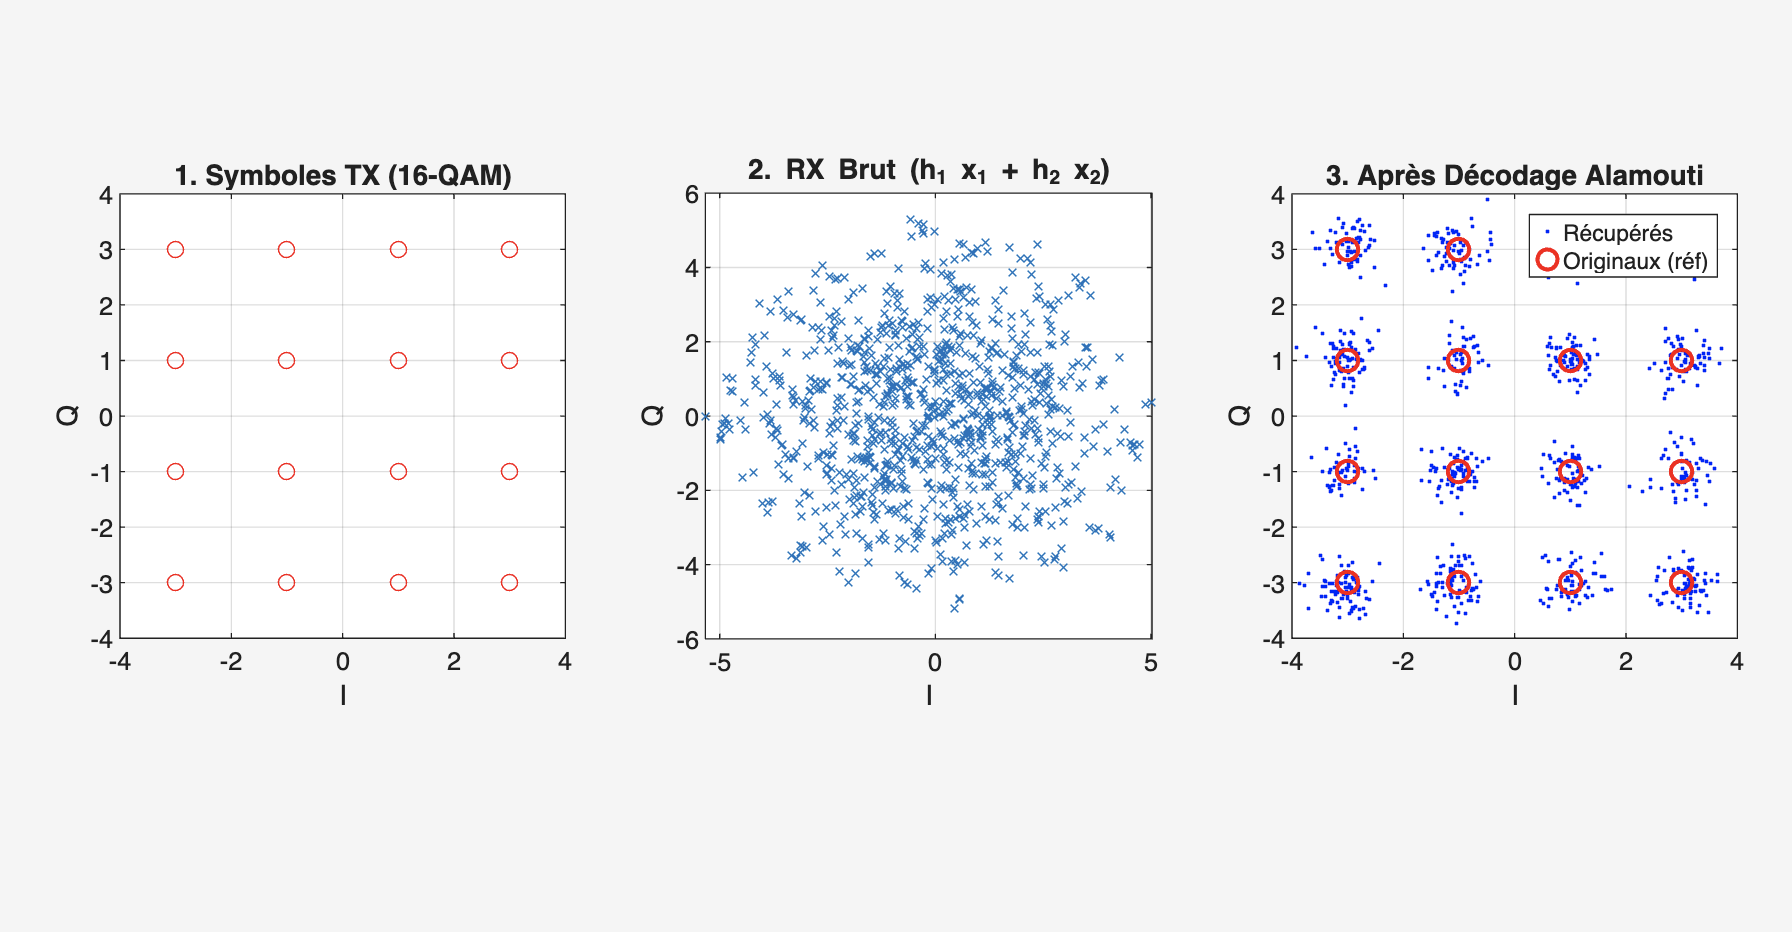
\includegraphics[width=0.85\textwidth, height=0.55\textheight, keepaspectratio]{Constellations_TX_RX_Decoded.png}
  \end{figure}
  
  \vspace{-0.5em}
  \begin{columns}
    \column{0.33\textwidth}
    \centering
    \footnotesize 1. TX: 16-QAM
    
    \column{0.33\textwidth}
    \centering
    \footnotesize 2. RX: $h_1 x_1 + h_2 x_2$
    
    \column{0.33\textwidth}
    \centering
    \footnotesize 3. After Alamouti Decoding
  \end{columns}
\end{frame}

\begin{frame}{BER Performance: SISO vs Alamouti}
  \begin{columns}
    \column{0.55\textwidth}
    \begin{figure}
      \centering
      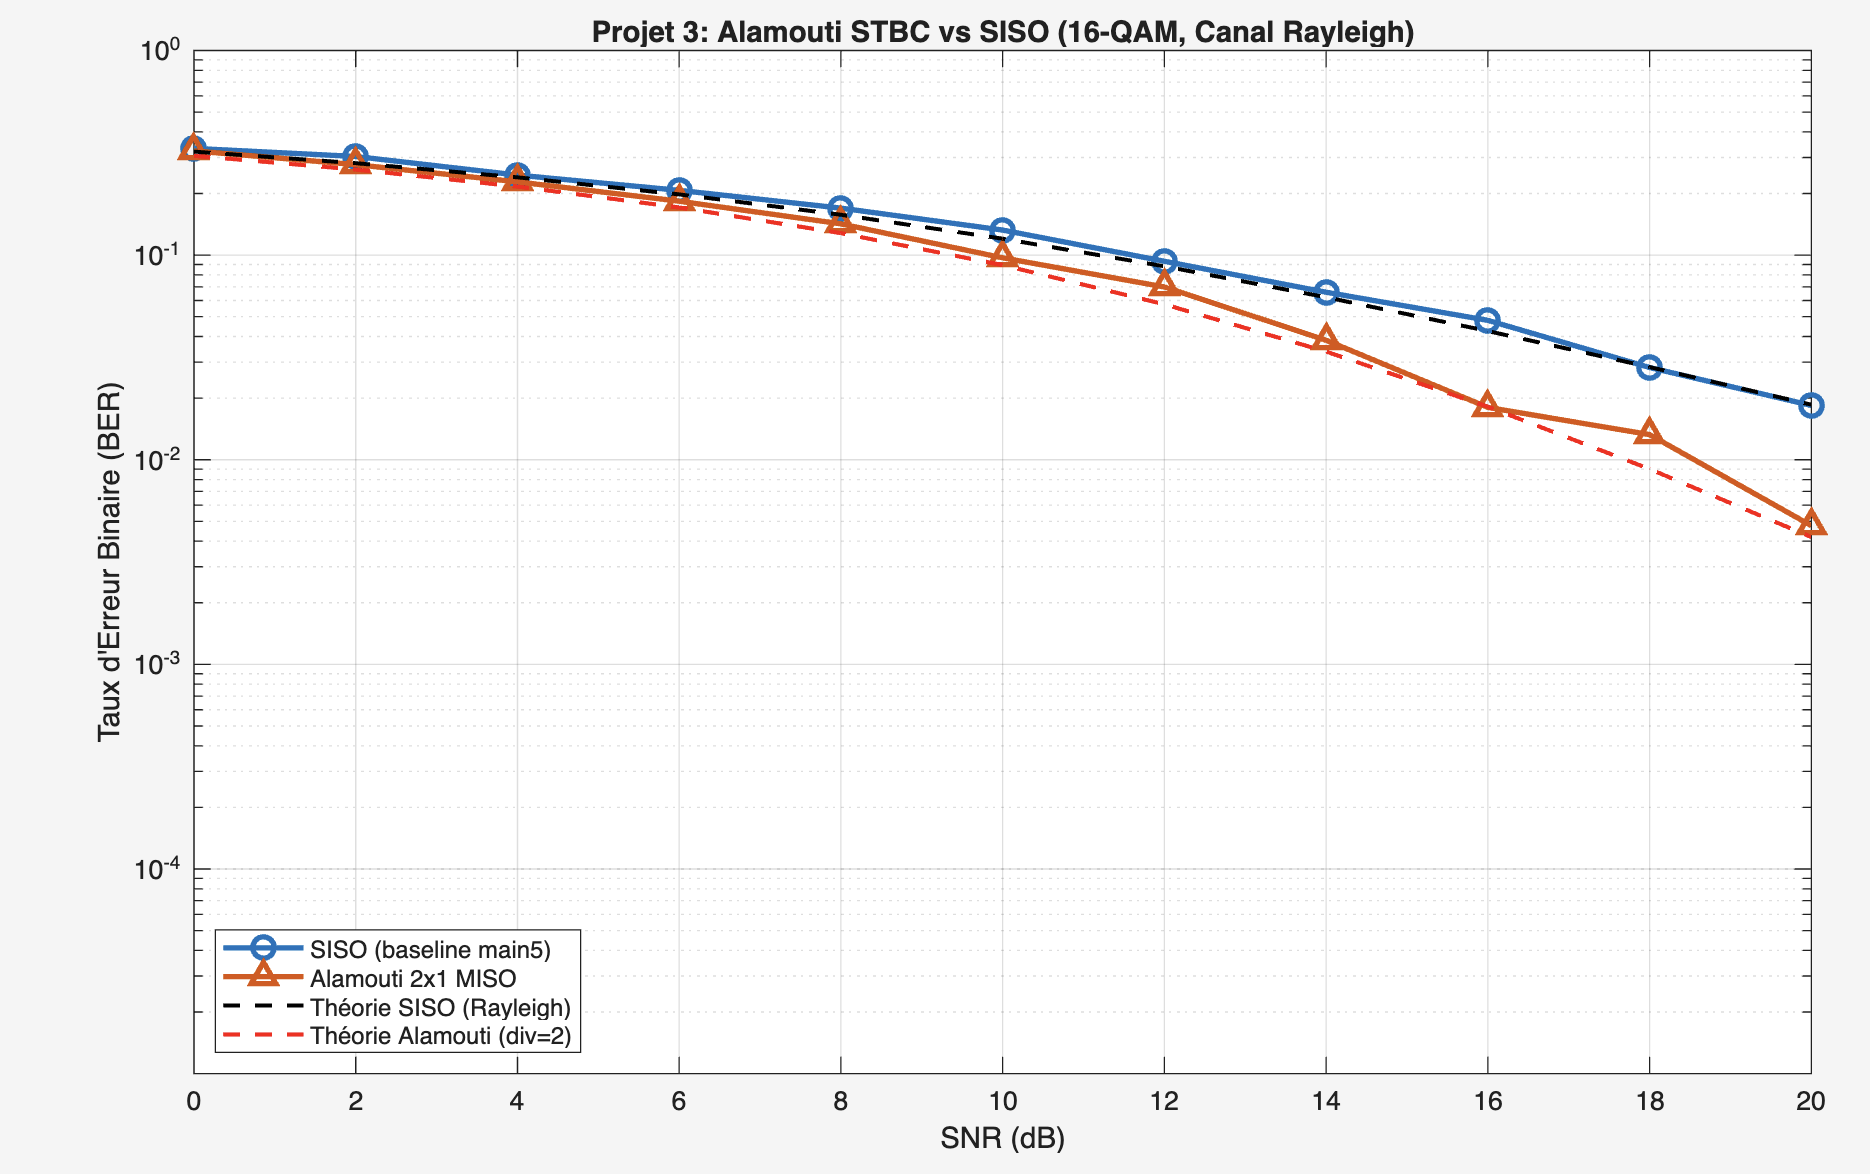
\includegraphics[width=\textwidth]{BER_Alamouti_vs_SISO_Rayleigh.png}
    \end{figure}
    
    \column{0.45\textwidth}
    \textbf{Key Observations:}
    \begin{itemize}
      \item Simulation matches theory
      \item Alamouti: steeper slope\\(diversity order = 2)
      \item \textbf{$\sim$4 dB gain} at BER $= 2\%$
    \end{itemize}
    
    \vspace{1em}
    \begin{block}{Diversity Gain}
      BER slope: $\propto \frac{1}{\text{SNR}^d}$\\
      SISO: $d=1$, Alamouti: $d=2$
    \end{block}
  \end{columns}
\end{frame}

% ============================================================
% ============================================================
% PART II: EXTENSIONS (Main_Alamouti_Extensions.m)
% ============================================================
% ============================================================

\section{Extensions: Overview}

\begin{frame}{Extension Project: Three Research Directions}
  \centering
  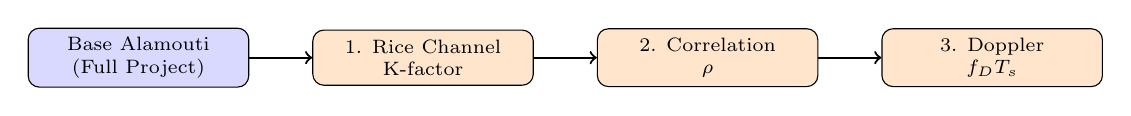
\begin{tikzpicture}[
    node distance=0.8cm,
    box/.style={rectangle, draw, rounded corners, minimum width=2.8cm, minimum height=0.7cm, align=center, font=\scriptsize},
    mainbox/.style={box, fill=blue!15},
    extbox/.style={box, fill=orange!20},
    arrow/.style={->, thick}
  ]
    \node[mainbox] (base) {Base Alamouti\\(Full Project)};
    \node[extbox, right=of base] (rice) {1. Rice Channel\\K-factor};
    \node[extbox, right=of rice] (corr) {2. Correlation\\$\rho$};
    \node[extbox, right=of corr] (dopp) {3. Doppler\\$f_DT_s$};
    
    \draw[arrow] (base) -- (rice);
    \draw[arrow] (rice) -- (corr);
    \draw[arrow] (corr) -- (dopp);
  \end{tikzpicture}
  
  \vspace{0.5em}
  \hrule
  \vspace{0.4em}
  
  \begin{columns}[t]
    \column{0.33\textwidth}
    \centering
    \textbf{\footnotesize Rice (K-factor)}
    
    \vspace{0.2em}
    \scriptsize
    \raggedright
    \textbf{Question:} How does LOS component affect performance?
    
    \vspace{0.2em}
    \textbf{Method:} Sweep K = 0, 5, 10 dB
    
    \vspace{0.2em}
    \textbf{Expected:} Higher K $\to$ lower BER
    
    \column{0.33\textwidth}
    \centering
    \textbf{\footnotesize Correlation ($\rho$)}
    
    \vspace{0.2em}
    \scriptsize
    \raggedright
    \textbf{Question:} What if antennas are too close?
    
    \vspace{0.2em}
    \textbf{Method:} Sweep $\rho$ = 0, 0.5, 0.9
    
    \vspace{0.2em}
    \textbf{Expected:} Higher $\rho$ $\to$ less diversity
    
    \column{0.33\textwidth}
    \centering
    \textbf{\footnotesize Doppler ($f_DT_s$)}
    
    \vspace{0.2em}
    \scriptsize
    \raggedright
    \textbf{Question:} What if user is moving fast?
    
    \vspace{0.2em}
    \textbf{Method:} Sweep $f_DT_s$ = 0 $\sim$ 0.02
    
    \vspace{0.2em}
    \textbf{Expected:} High Doppler $\to$ BER floor
  \end{columns}
\end{frame}

% ------------------------------------------------------------
\section{Extensions: Code Architecture}
% ------------------------------------------------------------

\begin{frame}{Extension Code: Overall Architecture}
  \begin{columns}
    \column{0.5\textwidth}
    \centering
    \textbf{Main Script Controls 3 Sweeps:}
    \vspace{0.5em}
    
    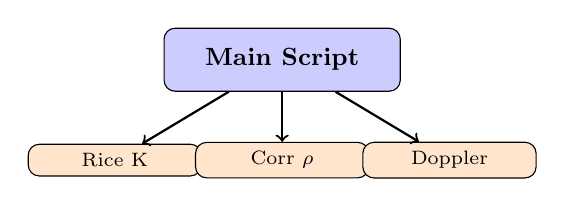
\begin{tikzpicture}[scale=0.85]
      % Main box
      \node[rectangle, draw, rounded corners, fill=blue!20, minimum width=3cm, minimum height=0.8cm, font=\small\bfseries] (main) at (0,0) {Main Script};
      
      % Three sweeps
      \node[rectangle, draw, rounded corners, fill=orange!20, minimum width=2.2cm, font=\scriptsize] (rice) at (-2.5,-1.5) {Rice K};
      \node[rectangle, draw, rounded corners, fill=orange!20, minimum width=2.2cm, font=\scriptsize] (corr) at (0,-1.5) {Corr $\rho$};
      \node[rectangle, draw, rounded corners, fill=orange!20, minimum width=2.2cm, font=\scriptsize] (dopp) at (2.5,-1.5) {Doppler};
      
      % Arrows
      \draw[->, thick] (main) -- (rice);
      \draw[->, thick] (main) -- (corr);
      \draw[->, thick] (main) -- (dopp);
    \end{tikzpicture}
    
    \column{0.5\textwidth}
    \centering
    \textbf{Two Local Functions:}
    \vspace{0.5em}
    
    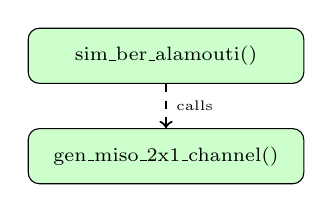
\begin{tikzpicture}[scale=0.85]
      % Function 1
      \node[rectangle, draw, rounded corners, fill=green!20, minimum width=3.5cm, minimum height=0.7cm, font=\scriptsize, align=center] (sim) at (0,0) {sim\_ber\_alamouti()};
      
      % Function 2
      \node[rectangle, draw, rounded corners, fill=green!20, minimum width=3.5cm, minimum height=0.7cm, font=\scriptsize, align=center] (gen) at (0,-1.5) {gen\_miso\_2x1\_channel()};
      
      % Arrow
      \draw[->, thick, dashed] (sim) -- node[right, font=\tiny] {calls} (gen);
    \end{tikzpicture}
  \end{columns}
  
  \vspace{0.8em}
  
  \begin{block}{Function Responsibilities}
    \small
    \begin{itemize}
      \item \textbf{sim\_ber\_alamouti()}: Complete TX-RX chain, two pilot modes, Monte Carlo BER
      \item \textbf{gen\_miso\_2x1\_channel()}: Rayleigh/Rice, spatial correlation, AR(1) Doppler
    \end{itemize}
  \end{block}
\end{frame}

\begin{frame}{Channel Configuration: Parameterized Design}
  \centering
  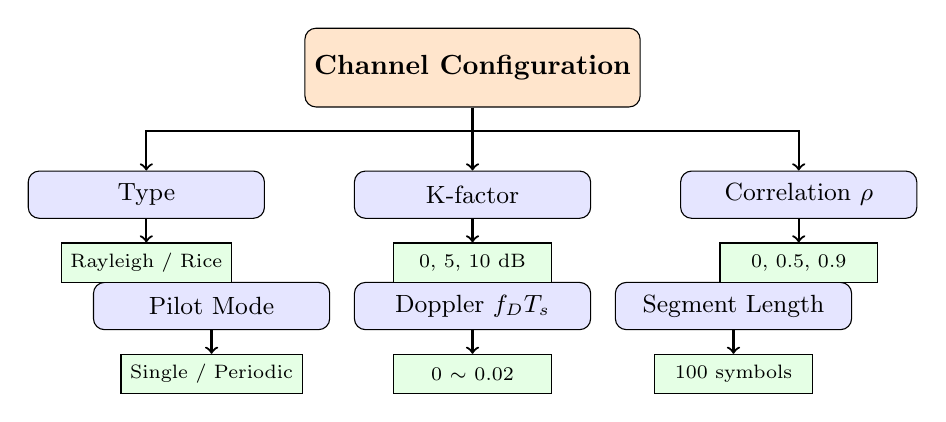
\begin{tikzpicture}[
    node distance=0.5cm,
    configbox/.style={rectangle, draw, rounded corners, fill=blue!10, minimum width=3cm, minimum height=0.6cm, align=center, font=\small},
    valuebox/.style={rectangle, draw, fill=green!10, minimum width=2cm, minimum height=0.5cm, align=center, font=\scriptsize},
    arrow/.style={->, thick}
  ]
    % Main config box
    \node[rectangle, draw, rounded corners, fill=orange!20, minimum width=4cm, minimum height=1cm, font=\bfseries] (chanopt) {Channel Configuration};
    
    % Parameters
    \node[configbox, below left=0.8cm and 0.5cm of chanopt] (type) {Type};
    \node[configbox, below=0.8cm of chanopt] (kfactor) {K-factor};
    \node[configbox, below right=0.8cm and 0.5cm of chanopt] (rho) {Correlation $\rho$};
    \node[configbox, below=0.8cm of kfactor] (fdts) {Doppler $f_DT_s$};
    \node[configbox, left=0.3cm of fdts] (pilot) {Pilot Mode};
    \node[configbox, right=0.3cm of fdts] (seglen) {Segment Length};
    
    % Values
    \node[valuebox, below=0.3cm of type] (typeval) {Rayleigh / Rice};
    \node[valuebox, below=0.3cm of kfactor] (kval) {0, 5, 10 dB};
    \node[valuebox, below=0.3cm of rho] (rhoval) {0, 0.5, 0.9};
    \node[valuebox, below=0.3cm of fdts] (fdval) {0 $\sim$ 0.02};
    \node[valuebox, below=0.3cm of pilot] (pilotval) {Single / Periodic};
    \node[valuebox, below=0.3cm of seglen] (segval) {100 symbols};
    
    % Arrows
    \draw[arrow] (chanopt.south) -- ++(0,-0.3) -| (type.north);
    \draw[arrow] (chanopt.south) -- (kfactor.north);
    \draw[arrow] (chanopt.south) -- ++(0,-0.3) -| (rho.north);
    
    \draw[arrow] (type) -- (typeval);
    \draw[arrow] (kfactor) -- (kval);
    \draw[arrow] (rho) -- (rhoval);
    \draw[arrow] (fdts) -- (fdval);
    \draw[arrow] (pilot) -- (pilotval);
    \draw[arrow] (seglen) -- (segval);
  \end{tikzpicture}
  
  \vspace{0.5em}
  \begin{block}{Design Philosophy}
    \small
    All channel parameters encapsulated in a single configuration structure, enabling flexible switching between different channel models \textbf{without modifying} core simulation logic.
  \end{block}
\end{frame}

\begin{frame}{Core Function: sim\_ber\_alamouti() Flow}
  \centering
  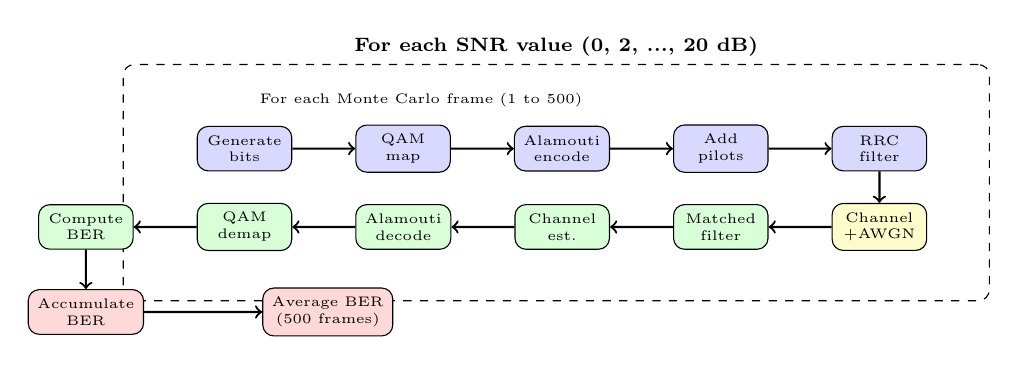
\begin{tikzpicture}[
    node distance=0.3cm and 0.8cm,
    box/.style={rectangle, draw, rounded corners, minimum width=1.2cm, minimum height=0.4cm, align=center, font=\tiny},
    loopbox/.style={rectangle, draw, dashed, rounded corners, minimum width=11cm, minimum height=3cm},
    arrow/.style={->, thick},
    scale=0.72
  ]
    % Outer loop label - above everything
    \node[font=\scriptsize\bfseries] (snrlabel) at (0, 1.2) {For each SNR value (0, 2, ..., 20 dB)};
    
    % Inner loop box - large enough to contain label and flow
    \node[loopbox] (innerloop) at (0, -1.2) {};
    
    % Inner loop label - inside the box at top left
    \node[font=\tiny, anchor=north west] at (-5.4, 0.55) {For each Monte Carlo frame (1 to 500)};
    
    % TX chain inside loop
    \node[box, fill=blue!15] at (-5.5, -0.6) (bits) {Generate\\bits};
    \node[box, fill=blue!15, right=of bits] (qam) {QAM\\map};
    \node[box, fill=blue!15, right=of qam] (alaenc) {Alamouti\\encode};
    \node[box, fill=blue!15, right=of alaenc] (pilot) {Add\\pilots};
    \node[box, fill=blue!15, right=of pilot] (rrc) {RRC\\filter};
    
    % Channel
    \node[box, fill=yellow!20, below=0.4cm of rrc] (ch) {Channel\\+AWGN};
    
    % RX chain
    \node[box, fill=green!15, left=of ch] (mf) {Matched\\filter};
    \node[box, fill=green!15, left=of mf] (chest) {Channel\\est.};
    \node[box, fill=green!15, left=of chest] (aladec) {Alamouti\\decode};
    \node[box, fill=green!15, left=of aladec] (deqam) {QAM\\demap};
    \node[box, fill=green!15, left=of deqam] (ber) {Compute\\BER};
    
    % Arrows
    \draw[arrow] (bits) -- (qam);
    \draw[arrow] (qam) -- (alaenc);
    \draw[arrow] (alaenc) -- (pilot);
    \draw[arrow] (pilot) -- (rrc);
    \draw[arrow] (rrc) -- (ch);
    \draw[arrow] (ch) -- (mf);
    \draw[arrow] (mf) -- (chest);
    \draw[arrow] (chest) -- (aladec);
    \draw[arrow] (aladec) -- (deqam);
    \draw[arrow] (deqam) -- (ber);
    
    % BER accumulate
    \node[box, fill=red!15, below=0.5cm of ber] (acc) {Accumulate\\BER};
    \draw[arrow] (ber) -- (acc);
    
    % Average
    \node[box, fill=red!15, right=1.5cm of acc] (avg) {Average BER\\(500 frames)};
    \draw[arrow] (acc) -- (avg);
  \end{tikzpicture}
  
  \vspace{0.3em}
  \small
  \textbf{Output}: BER array of length 11, one value per SNR point
\end{frame}

\begin{frame}{Two Pilot Modes: Single vs Periodic}
  \begin{columns}
    \column{0.5\textwidth}
    \centering
    \textbf{\large Single Pilot Mode}
    
    \vspace{0.5em}
    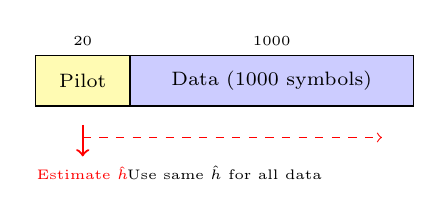
\begin{tikzpicture}[scale=0.8]
      % Frame structure
      \draw[fill=yellow!30] (0,0) rectangle (1.5,0.8);
      \node at (0.75,0.4) {\scriptsize Pilot};
      \draw[fill=blue!20] (1.5,0) rectangle (6,0.8);
      \node at (3.75,0.4) {\scriptsize Data (1000 symbols)};
      
      % Labels
      \node[above] at (0.75,0.8) {\tiny 20};
      \node[above] at (3.75,0.8) {\tiny 1000};
      
      % Channel estimation arrow
      \draw[->, thick, red] (0.75,-0.3) -- (0.75,-0.8) node[below, font=\tiny] {Estimate $\hat{h}$};
      \draw[->, dashed, red] (0.75,-0.5) -- (5.5,-0.5);
      \node[below, font=\tiny] at (3,-0.8) {Use same $\hat{h}$ for all data};
    \end{tikzpicture}
    
    \vspace{0.5em}
    \begin{itemize}
      \scriptsize
      \item Channel estimated \textbf{once} at frame start
      \item Low overhead (20/1020 = 2\%)
      \item \textcolor{red}{Problem}: If channel varies, estimate becomes outdated
    \end{itemize}
    
    \column{0.5\textwidth}
    \centering
    \textbf{\large Periodic Pilot Mode}
    
    \vspace{0.5em}
    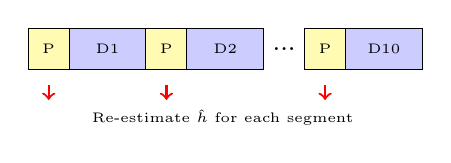
\begin{tikzpicture}[scale=0.65]
      % Segment 1
      \draw[fill=yellow!30] (0,0) rectangle (0.8,0.8);
      \node at (0.4,0.4) {\tiny P};
      \draw[fill=blue!20] (0.8,0) rectangle (2.3,0.8);
      \node at (1.55,0.4) {\tiny D1};
      
      % Segment 2
      \draw[fill=yellow!30] (2.3,0) rectangle (3.1,0.8);
      \node at (2.7,0.4) {\tiny P};
      \draw[fill=blue!20] (3.1,0) rectangle (4.6,0.8);
      \node at (3.85,0.4) {\tiny D2};
      
      % Dots
      \node at (5,0.4) {...};
      
      % Segment N
      \draw[fill=yellow!30] (5.4,0) rectangle (6.2,0.8);
      \node at (5.8,0.4) {\tiny P};
      \draw[fill=blue!20] (6.2,0) rectangle (7.7,0.8);
      \node at (6.95,0.4) {\tiny D10};
      
      % Channel estimation arrows
      \draw[->, thick, red] (0.4,-0.3) -- (0.4,-0.6);
      \draw[->, thick, red] (2.7,-0.3) -- (2.7,-0.6);
      \draw[->, thick, red] (5.8,-0.3) -- (5.8,-0.6);
      \node[below, font=\tiny] at (3.8,-0.6) {Re-estimate $\hat{h}$ for each segment};
    \end{tikzpicture}
    
    \vspace{0.5em}
    \begin{itemize}
      \scriptsize
      \item Channel estimated \textbf{every segment}
      \item Higher overhead (200/1200 = 17\%)
      \item \textcolor{green!50!black}{Benefit}: Tracks time-varying channels
    \end{itemize}
  \end{columns}
  
  \vspace{0.5em}
  \hrule
  \vspace{0.3em}
  \centering
  \small
  \textbf{Selection Rule}: Use \textit{Single} for static channels ($f_DT_s = 0$), \textit{Periodic} for Doppler scenarios
\end{frame}

\begin{frame}{Channel Generation: Detailed Algorithm}
  \begin{columns}
    \column{0.4\textwidth}
    \centering
    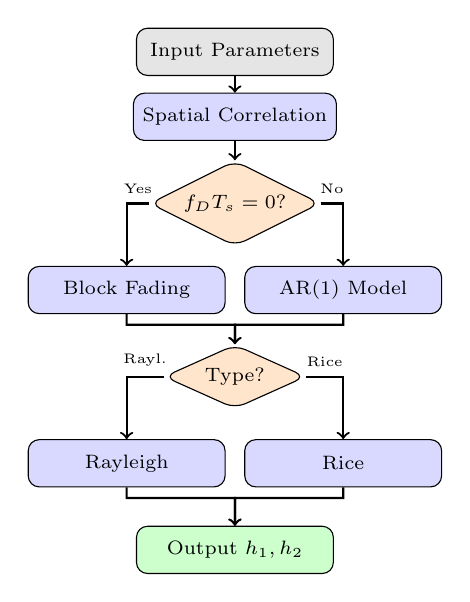
\begin{tikzpicture}[
      scale=0.55,
      every node/.style={font=\scriptsize},
      box/.style={rectangle, draw, rounded corners, minimum height=0.6cm, minimum width=2.5cm, align=center},
      inputbox/.style={box, fill=gray!20},
      procbox/.style={box, fill=blue!15},
      decbox/.style={box, fill=orange!20, diamond, aspect=2, inner sep=2pt, minimum width=1.8cm},
      outbox/.style={box, fill=green!20},
      arrow/.style={->, thick}
    ]
      % Row 0: Input
      \node[inputbox] (input) at (0,0) {Input Parameters};
      
      % Row 1: Spatial Correlation
      \node[procbox] (corr) at (0,-1.5) {Spatial Correlation};
      
      % Row 2: Doppler decision
      \node[decbox] (dopp) at (0,-3.5) {$f_DT_s=0$?};
      
      % Row 3: Block / AR(1)
      \node[procbox] (block) at (-2.5,-5.5) {Block Fading};
      \node[procbox] (ar1) at (2.5,-5.5) {AR(1) Model};
      
      % Row 4: Type decision
      \node[decbox] (type) at (0,-7.5) {Type?};
      
      % Row 5: Rayleigh / Rice
      \node[procbox] (rayl) at (-2.5,-9.5) {Rayleigh};
      \node[procbox] (rice) at (2.5,-9.5) {Rice};
      
      % Row 6: Output
      \node[outbox] (out) at (0,-11.5) {Output $h_1, h_2$};
      
      % === ARROWS ===
      % Main vertical flow
      \draw[arrow] (input) -- (corr);
      \draw[arrow] (corr) -- (dopp);
      
      % Doppler decision: split left/right
      \draw[arrow] (dopp) -| node[pos=0.25, above, font=\tiny] {Yes} (block);
      \draw[arrow] (dopp) -| node[pos=0.25, above, font=\tiny] {No} (ar1);
      
      % Block and AR(1) merge into Type (via top)
      \draw[arrow] (block) -- ++(0,-0.8) -| (type);
      \draw[arrow] (ar1) -- ++(0,-0.8) -| (type);
      
      % Type decision: split left/right
      \draw[arrow] (type) -| node[pos=0.25, above, font=\tiny] {Rayl.} (rayl);
      \draw[arrow] (type) -| node[pos=0.25, above, font=\tiny] {Rice} (rice);
      
      % Rayleigh and Rice merge into Output (via top)
      \draw[arrow] (rayl) -- ++(0,-0.8) -| (out);
      \draw[arrow] (rice) -- ++(0,-0.8) -| (out);
    \end{tikzpicture}
    
    \column{0.6\textwidth}
    \small
    \textbf{Step 1: Spatial Correlation}
    \begin{itemize}
      \scriptsize
      \item Build: $\mathbf{R} = \begin{bmatrix} 1 & \rho \\ \rho & 1 \end{bmatrix}$
      \item Cholesky: $\mathbf{L} = \text{chol}(\mathbf{R})$
      \item Generate: $\mathbf{U} \sim \mathcal{CN}(0,1)$
      \item Correlate: $\mathbf{W} = \mathbf{L} \cdot \mathbf{U}$
    \end{itemize}
    
    \vspace{0.3em}
    \textbf{Step 2: Doppler (Time Variation)}
    \begin{itemize}
      \scriptsize
      \item \textbf{Block} ($f_DT_s=0$): $h[n] = h[1]$ (constant)
      \item \textbf{AR(1)} ($f_DT_s>0$): $h[n] = a \cdot h[n-1] + b \cdot w[n]$\\
            where $a = J_0(2\pi f_D T_s)$, $b = \sqrt{1-a^2}$
    \end{itemize}
    
    \vspace{0.3em}
    \textbf{Step 3: Channel Type}
    \begin{itemize}
      \scriptsize
      \item \textbf{Rayleigh}: $H = H_{\text{NLOS}}$
      \item \textbf{Rice}: $H = \sqrt{\frac{K}{1+K}}H_{\text{LOS}} + \sqrt{\frac{1}{1+K}}H_{\text{NLOS}}$
    \end{itemize}
  \end{columns}
\end{frame}

% ------------------------------------------------------------
\section{Extensions: Results}
% ------------------------------------------------------------

\begin{frame}{Extension 1: Rice Channel (K-Factor)}
  \begin{columns}
    \column{0.55\textwidth}
    \begin{figure}
      \centering
      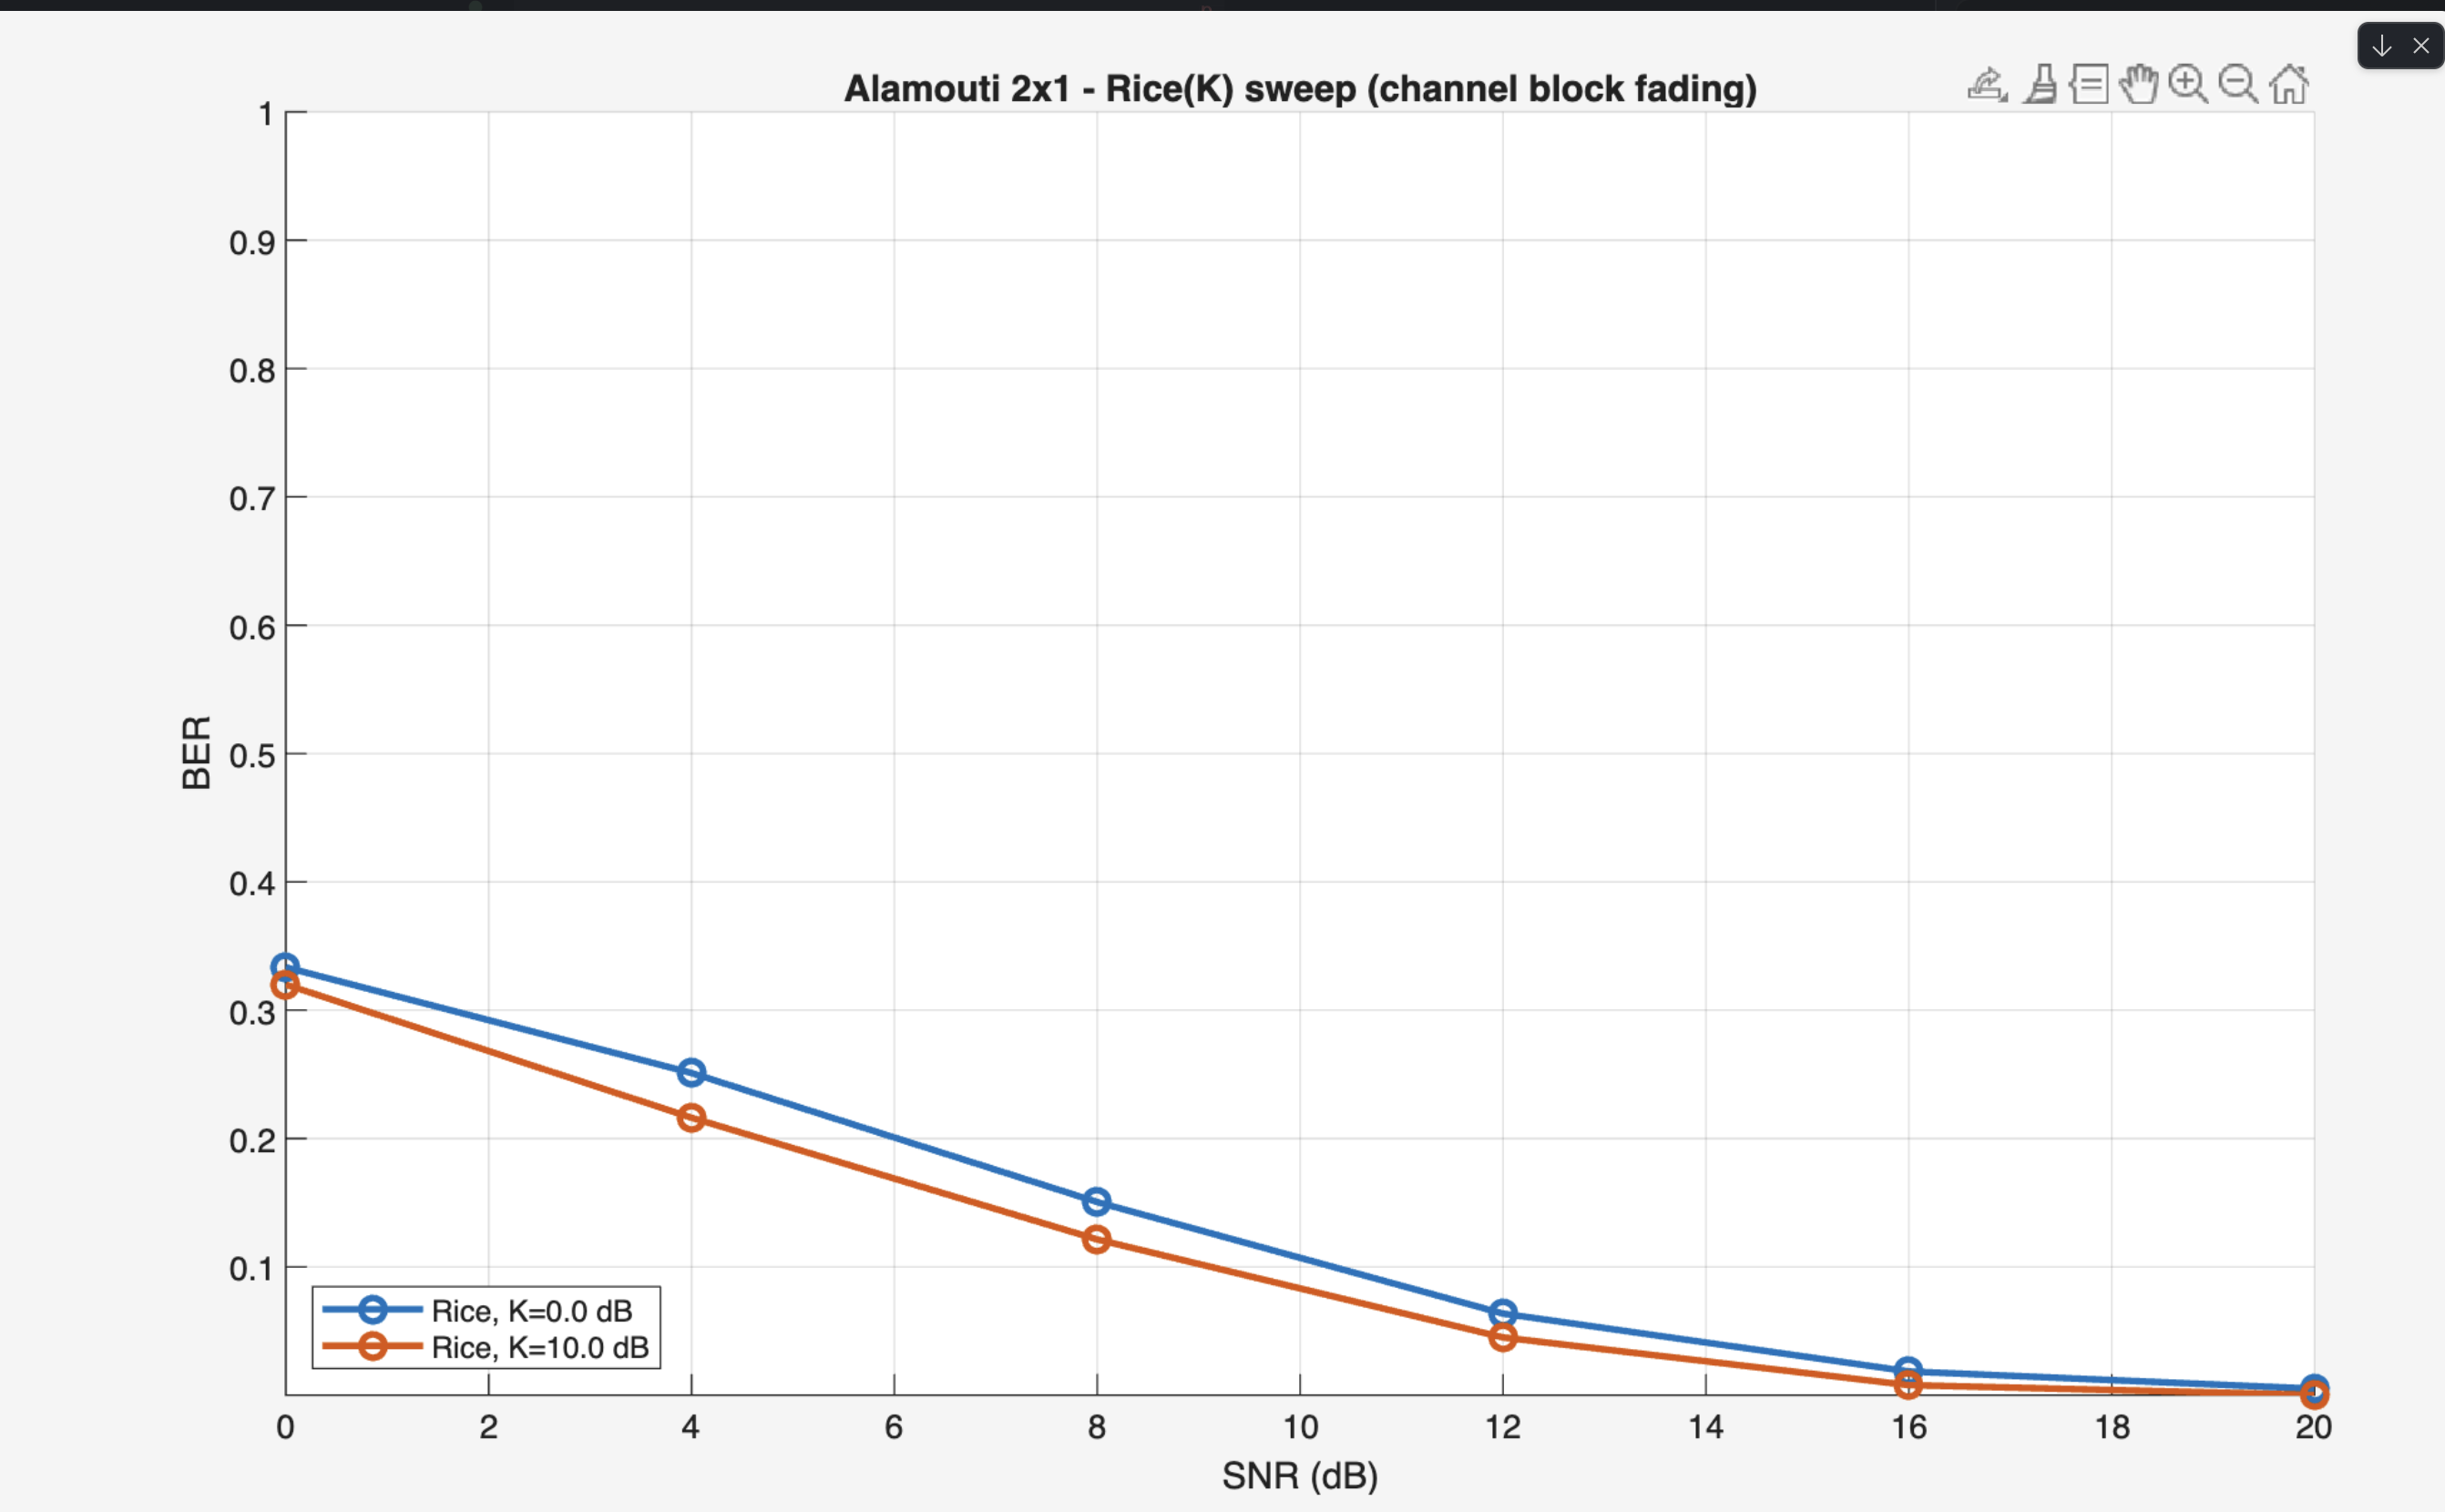
\includegraphics[width=\textwidth]{RICE(K).png}
    \end{figure}
    
    \column{0.45\textwidth}
    \textbf{Rice Channel Model:}
    \[
    h = \sqrt{\frac{K}{1+K}} h_{\text{LOS}} + \sqrt{\frac{1}{1+K}} h_{\text{NLOS}}
    \]
    
    \vspace{0.5em}
    \textbf{Observation:}
    \begin{itemize}
      \item Higher K $\Rightarrow$ Stronger LOS
      \item Higher K $\Rightarrow$ Lower BER
      \item Less deep fading
    \end{itemize}
    
    \vspace{0.5em}
    \textbf{K values tested:}\\
    0 dB (Rayleigh), 5 dB, 10 dB
  \end{columns}
\end{frame}

\begin{frame}{Extension 2: TX Spatial Correlation ($\rho$)}
  \begin{columns}
    \column{0.55\textwidth}
    \begin{figure}
      \centering
      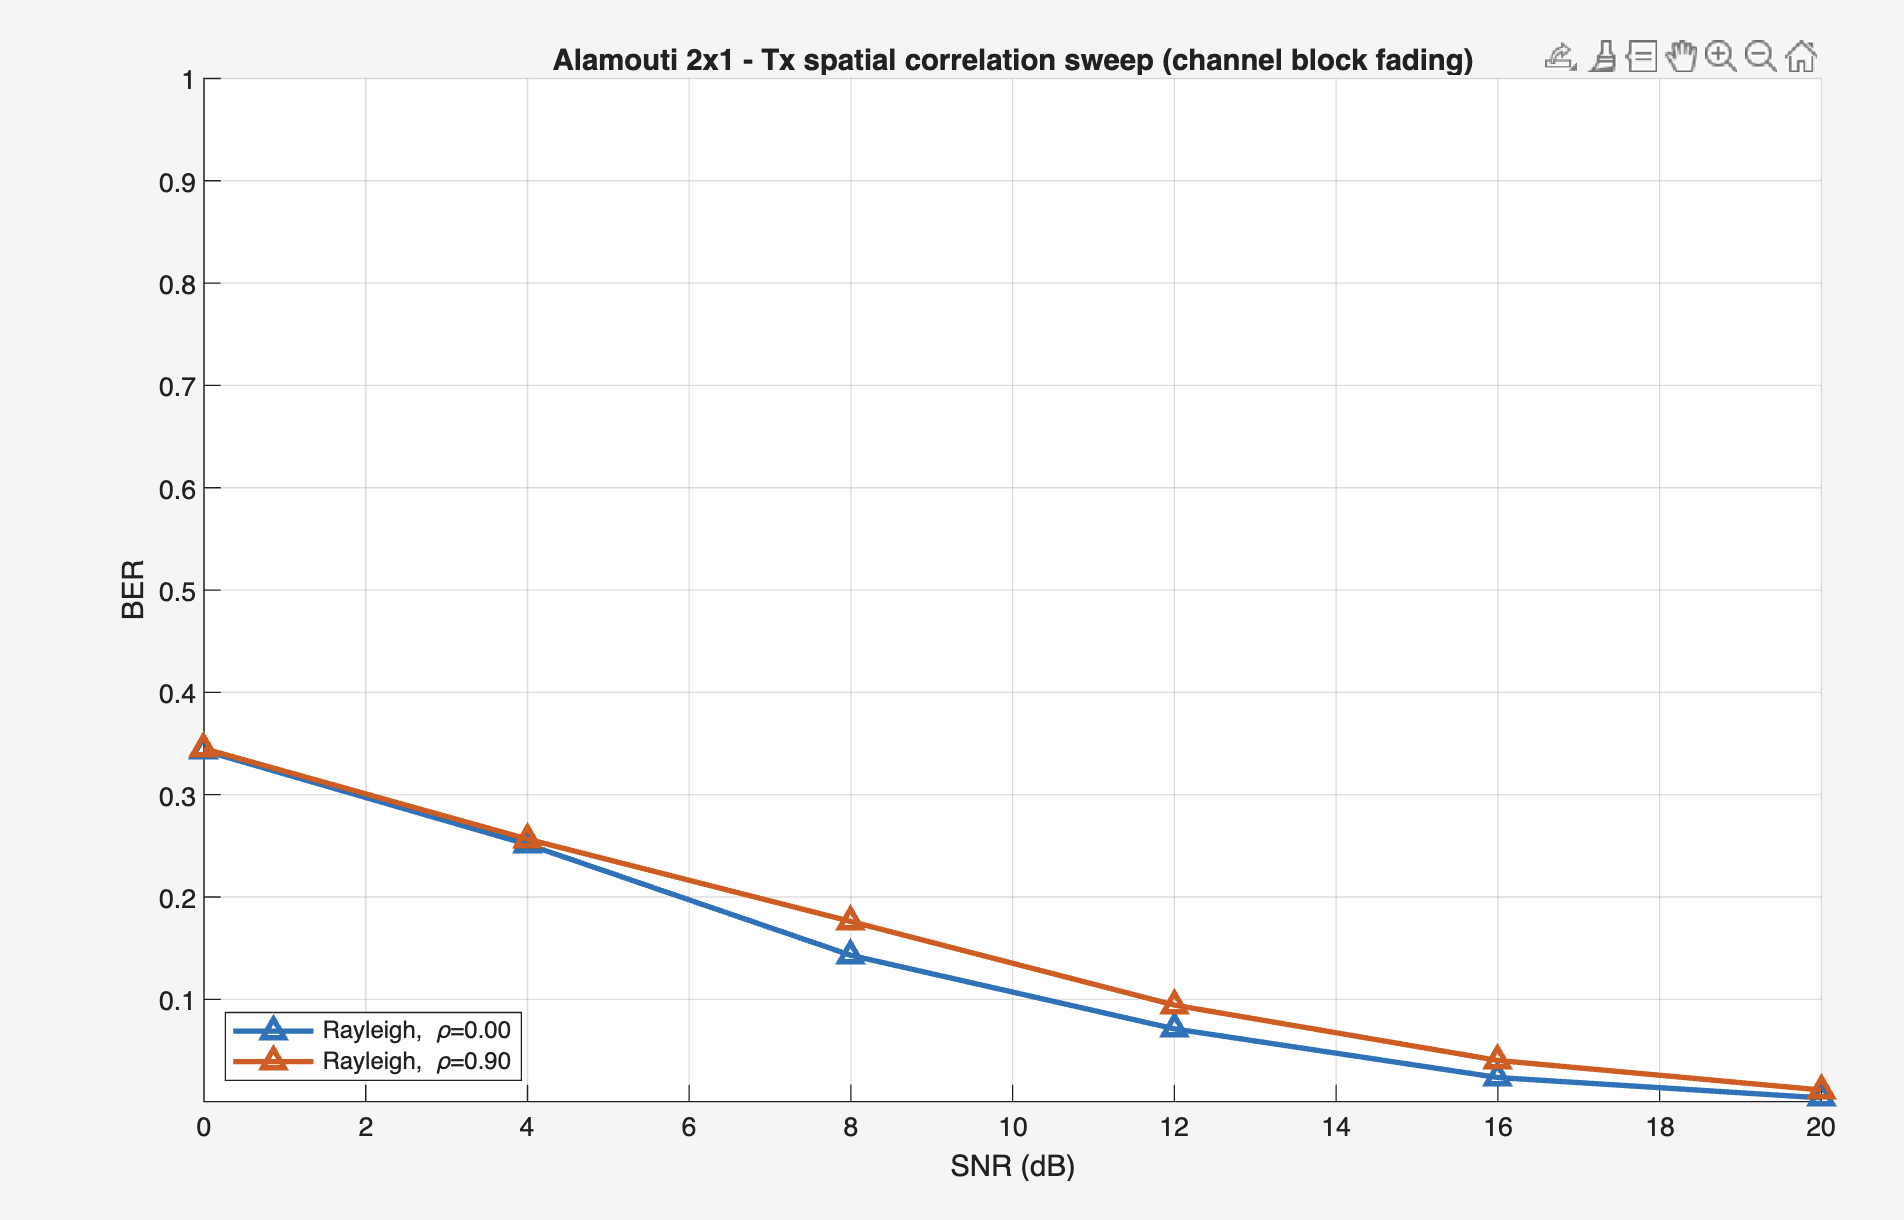
\includegraphics[width=\textwidth]{corre.png}
    \end{figure}
    
    \column{0.45\textwidth}
    \textbf{Correlation Model:}
    \[
    \mathbf{R} = \begin{bmatrix} 1 & \rho \\ \rho & 1 \end{bmatrix}, \quad \mathbf{H} = \mathbf{L}\mathbf{U}
    \]
    
    \vspace{0.5em}
    \textbf{Observation:}
    \begin{itemize}
      \item Higher $\rho$ $\Rightarrow$ $h_1 \approx h_2$
      \item Diversity gain reduced
      \item $\rho = 0$: Independent (ideal)
      \item $\rho \to 1$: No diversity
    \end{itemize}
    
    \vspace{0.5em}
    \textbf{$\rho$ values tested:}\\
    0, 0.5, 0.9
  \end{columns}
\end{frame}

\begin{frame}{Extension 3: Doppler Time-Varying Fading}
  \begin{columns}
    \column{0.55\textwidth}
    \begin{figure}
      \centering
      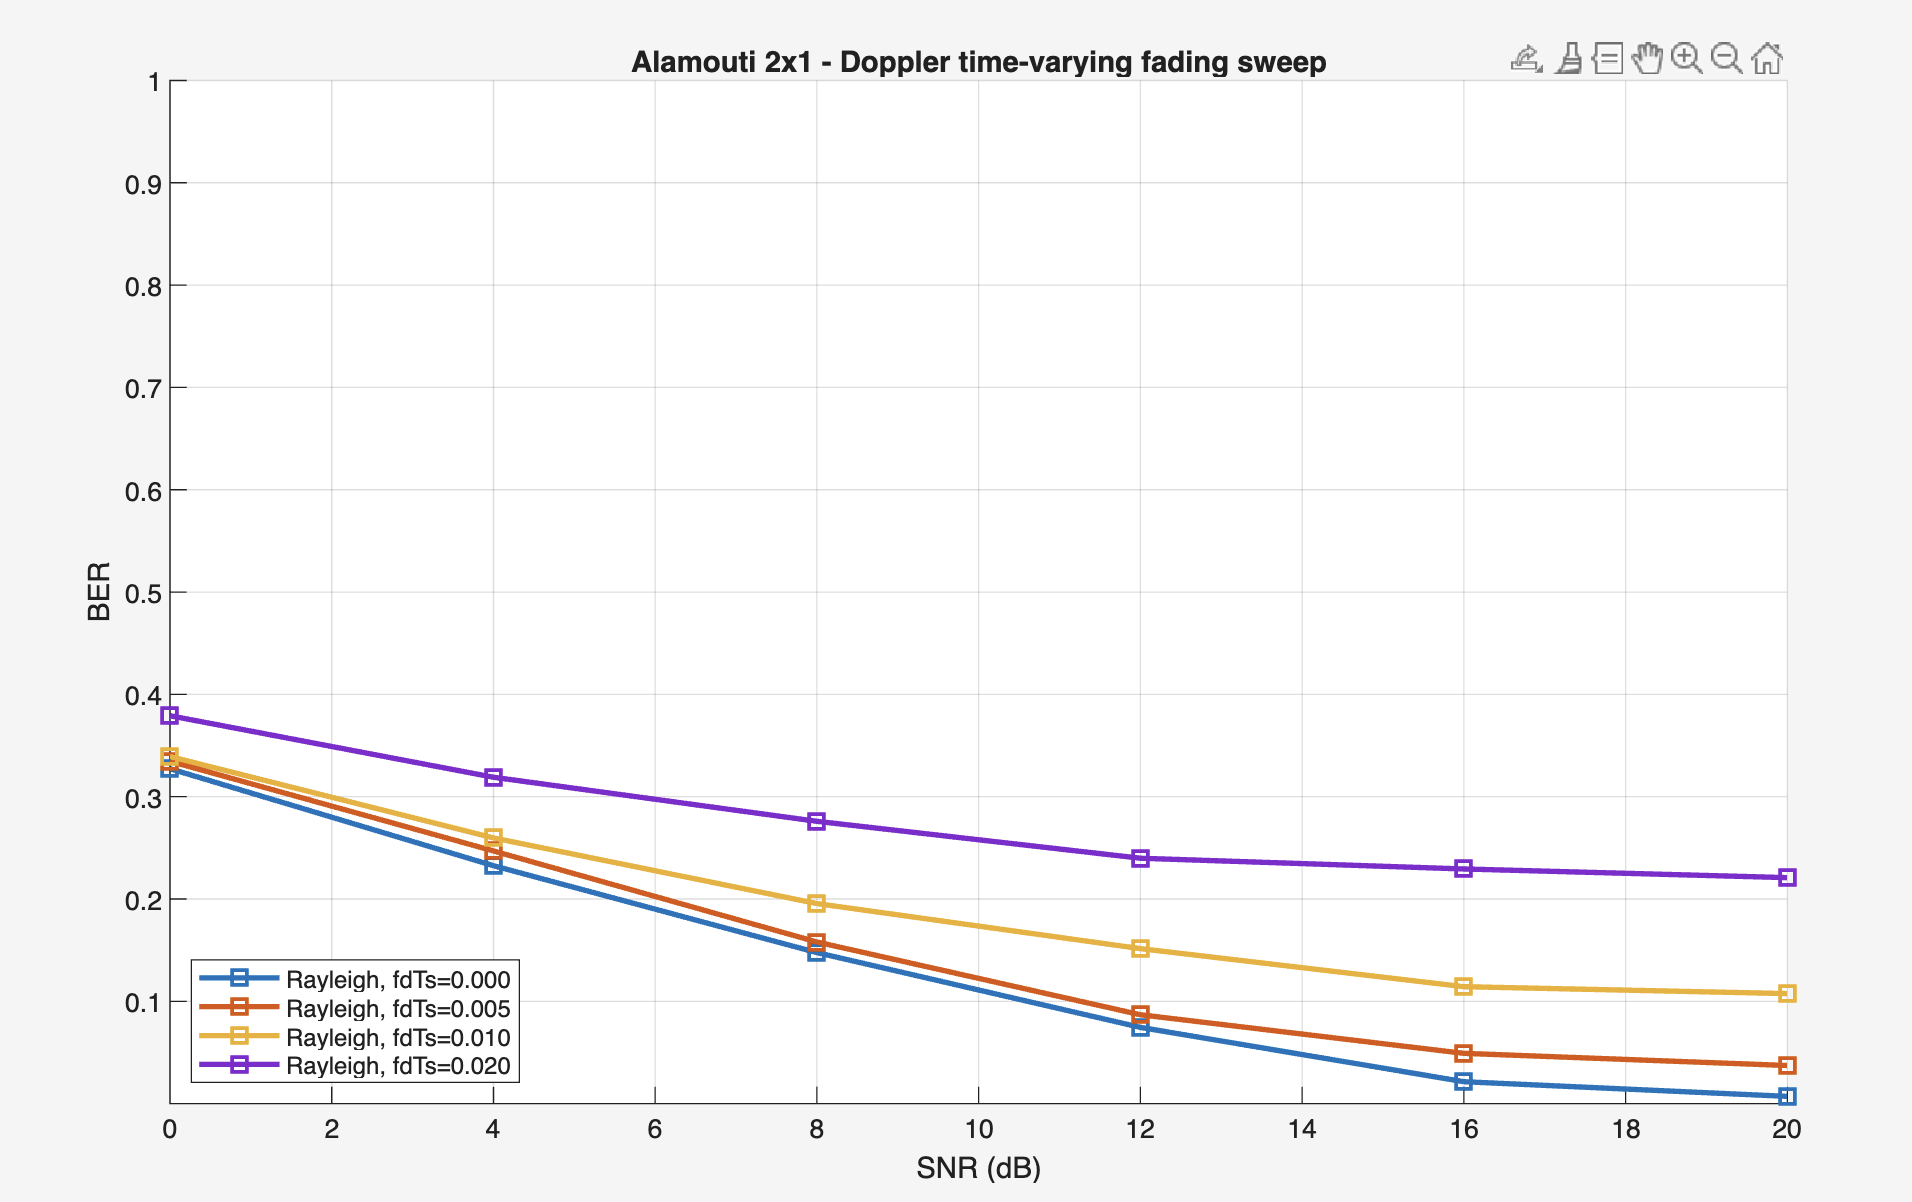
\includegraphics[width=\textwidth]{Doppler.png}
    \end{figure}
    
    \column{0.45\textwidth}
    \textbf{AR(1) Model:}
    \[
    h[n] = a \cdot h[n-1] + b \cdot w[n]
    \]
    where $a = J_0(2\pi f_D T_s)$, $b = \sqrt{1-a^2}$
    
    \vspace{0.5em}
    \textbf{Observation:}
    \begin{itemize}
      \item Higher $f_D T_s$ $\Rightarrow$ Faster variation
      \item Alamouti assumes $h$ constant over 2 slots
      \item High Doppler $\Rightarrow$ BER floor
    \end{itemize}
    
    \vspace{0.5em}
    \textbf{Solution:}\\
    Periodic pilot tracking
  \end{columns}
\end{frame}

% ============================================================
\section{Conclusion}
% ============================================================

\begin{frame}{Conclusion}
  \begin{columns}
    \column{0.5\textwidth}
    \textbf{Base Project:}
    \begin{itemize}
      \item[$\checkmark$] Implemented Alamouti 2×1 MISO
      \item[$\checkmark$] 16-QAM + pilot-based estimation
      \item[$\checkmark$] BER matches theoretical curves
      \item[$\checkmark$] $\sim$4 dB gain over SISO
    \end{itemize}
    
    \vspace{1em}
    \textbf{Extensions:}
    \begin{itemize}
      \item[$\checkmark$] Rice channel (K-factor)
      \item[$\checkmark$] Spatial correlation ($\rho$)
      \item[$\checkmark$] Doppler fading with periodic tracking
    \end{itemize}
    
    \column{0.5\textwidth}
    \begin{block}{Key Takeaways}
      \begin{enumerate}
        \item Alamouti achieves \textbf{full diversity} (order 2) with simple linear decoder
        \item Performance degrades with:
        \begin{itemize}
          \item High antenna correlation
          \item Fast time-varying channels
        \end{itemize}
        \item Rice channel improves performance (LOS)
        \item \textbf{Periodic pilots} essential for Doppler scenarios
      \end{enumerate}
    \end{block}
  \end{columns}
\end{frame}

\begin{frame}
  \centering
  \Huge \textbf{Thank You!}
  
  \vspace{2em}
  \Large Questions?
  
  \vspace{2em}
  \normalsize
  Code available at:\\
  \url{https://github.com/vimboom123/tp_com}
\end{frame}

\end{document}
